\subsection{Neural Network}
Neural Collaborative filtering attempts to find recommendations similar to those provided by the matrix
factorization on SVD, but powered by the versatility of neural networks.\\
As mentioned previously, we are trying to get a prediction for the score of a movie, for a given user.
That is, we want to feed the model a user and a movie and get a predicted score.\\
\subsubsection*{Network Modeling}
Our Neural Collaborative Filter receives a user and a movie (\emph{Input}) and generates an \emph{Embedding} for each of them.\\
Designing the Neural Network would take much research and experimenting; given our short deadline, we chose to use a tested one
(Wittenauer, 2019\footnote{\href{https://medium.com/@jdwittenauer/deep-learning-with-keras-recommender-systems-e7b99cb29929}{https://medium.com/@jdwittenauer/deep-learning-with-keras-recommender-systems-e7b99cb29929}}).
It involves a sequence of layers and dropouts, following the pattern:
\begin{center}
    \emph{Dropout (5\%) - 10 Fully Connected (FC) Neurons with ReLU activation - Dropout (10\%) - 1 FC Neuron with sigmoid activation - Scaling to prediction range (1-5) = result}\\
\end{center}
\begin{center}
    \captionsetup{type=figure}
    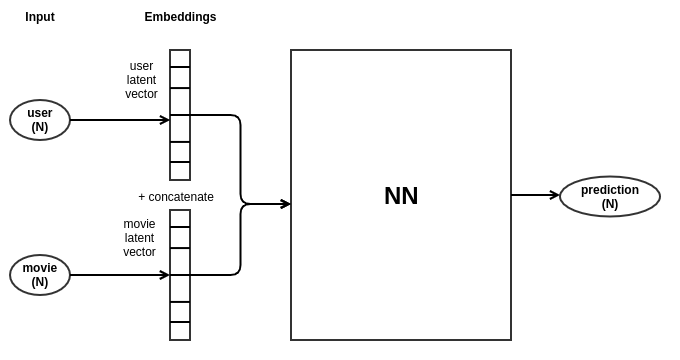
\includegraphics[width=250px]{images/nn-model.png}
    \captionof{figure}{Neural Collaborative Filter Model}
\end{center}

\subsubsection*{Implementation}
For this problem, considering our available time and the high level of abstraction of the library, we decide to use \emph{keras}.
\footnote{\href{https://keras.io/examples/structured\_data/collaborative\_filtering\_movielens/}{https://keras.io/examples/structured\_data/collaborative\_filtering\_movielens/}}
Again, modularizing the problem into functions is the proper solution for us:
\begin{enumerate}
    \item Generate the predictor
    \item Predict scores (given user-movie pairs)
    \item Get top predictions
\end{enumerate}
\subsubsection*{Generate Model}
To generate and train the model we migrate our model directly to the tools provided by keras.
The chosen cost function to optimize is Mean Squared Error.\\
The learning curve obtained by training our small dataset shows a tendency to overfit quickly (after 4 epochs).
Using the large dataset would probably solve this partially, but our resources for this study are limited
and doing so would take over a week (each epoch shows an estimated time of fourteen hours, and 8 epochs are not enough for 26 million inputs)
\begin{center}
    \captionsetup{type=figure}
    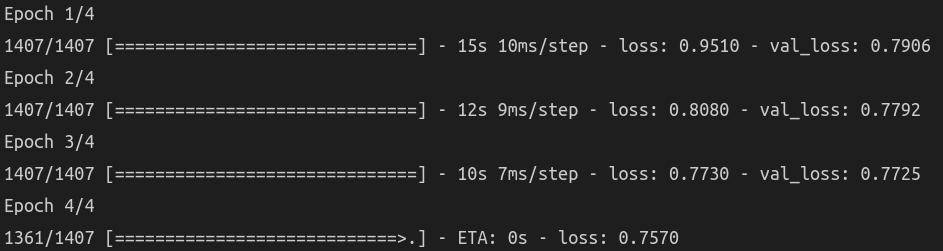
\includegraphics[width=250px]{images/nn-train-sm.png}
    \captionof{figure}{Training the Neural Network}
\end{center}
\begin{center}
    \captionsetup{type=figure}
    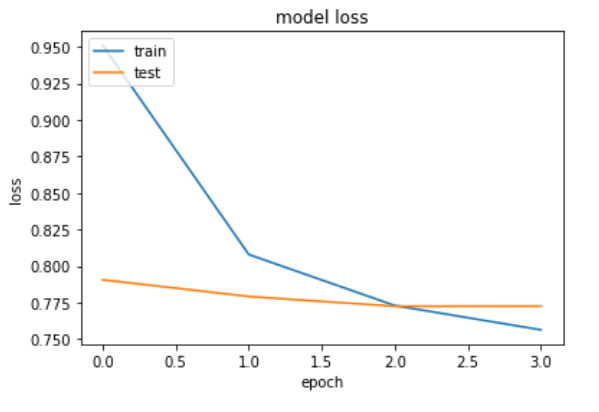
\includegraphics[width=250px]{images/nn-learn.png}
    \captionof{figure}{Learning Curve - Small Dataset}
\end{center}
After making it fit our data, we serialize the generated model using the builtin keras' save() method,
and from now on we don't need to generate it anymore, but just deserialize it and use it.

\subsubsection*{Predict Scores}
Predicting scores involves sending the users and movies lists to the model, and waiting for its answer.

\subsubsection*{Get Top Predictions}
From the nature of the Neural Collaborative Filter, all movies can be sent to the model to get a list of predictions for the same user (sending the user once per movie).\\
Finally, we are able to use this list, order it by prediction value (descending) and take the best 10 movies as our final result.
\begin{center}
    \captionsetup{type=figure}
    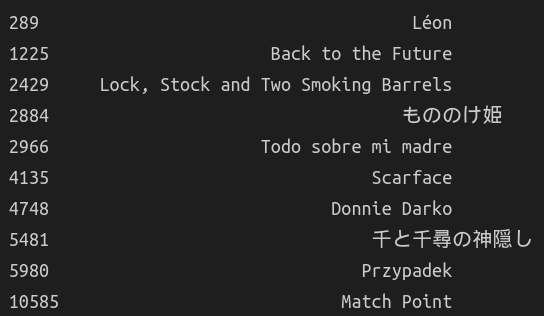
\includegraphics[width=250px]{images/nn-top.png}
    \captionof{figure}{NN: top 10 predictions for user}
\end{center}
